\printnomenclature[3.5cm] % Значение ширины столбца с обозначениями стоит подбирать вручную

\newpage

\begin{figure}[ht]
    \centerfloat{
        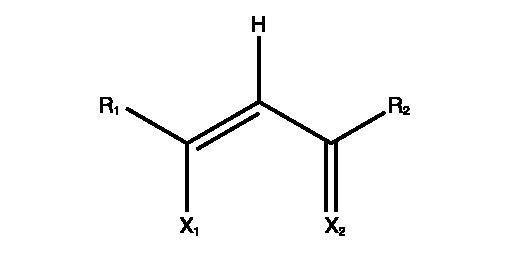
\includegraphics[scale=1.25]{stroenie-beta.pdf}
    }
\label{fig:latex}
\end{figure}

\begin{table} [htbp]%
    \centering
    \caption{Исследованные соединения}%
    \label{tab:test1}% 
    \renewcommand{\arraystretch}{1.5}%% Увеличение расстояния между рядами, для улучшения восприятия.
    \begin{SingleSpace}
        \begin{tabular}{@{}@{\extracolsep{20pt}}lllll@{}} %Вертикальные полосы не используются принципиально, как и лишние горизонтальные (допускается по ГОСТ 2.105 пункт 4.4.5) % @{} позволяет прижиматься к краям
            \toprule     %%% верхняя линейка
            Compound & X$_1$      & X$_2$  & R$_1$      & R$_2$      \\
            \midrule 
            I        & H          & O      & H          & H          \\
            II       & H          & O      & CH$_3$     & CH$_3$     \\
            III      & NH$_2$     & O      & CH$_3$     & CH$_3$     \\
            IV       & NHCH$_3$   & O      & CH$_3$     & CH$_3$     \\
            V        & SCH$_3$    & O      & CH$_3$     & CH$_3$     \\
            VI       & SH         & O      & CH$_3$     & CH$_3$     \\
            VII      & OH         & S      & CH$_3$     & CH$_3$     \\
            VIII     & OH         & O      & CF$_3$     & CH$_3$     \\
            IX       & OH         & O      & CF$_3$     & CF$_3$     \\
            X        & OH         & O      & C$_6$H$_5$ & C$_6$H$_5$ \\
            \bottomrule 
        \end{tabular}
    \end{SingleSpace}
\end{table}
